\documentclass{article}%
\usepackage[T1]{fontenc}%
\usepackage[utf8]{inputenc}%
\usepackage{lmodern}%
\usepackage{textcomp}%
\usepackage{lastpage}%
\usepackage[head=40pt,margin=0.5in,bottom=0.6in]{geometry}%
\usepackage{graphicx}%
%
\title{\textbf{Retenidos al menos 15 “garimpeiros” del río Guaire por PNB}}%
\author{Diario El Universal}%
\date{02/04/2018}%
%
\begin{document}%
\normalsize%
\maketitle%
\textbf{URL: }%
http://www.eluniversal.com/sucesos/4672/retenidos{-}menos{-}garimpeiros?{-}guaire\newline%
%
\textbf{Periodico: }%
EU, %
ID: %
4672, %
Seccion: %
sucesos\newline%
%
\textbf{Palabras Claves: }%
NO\_TIENE\newline%
%
\textbf{Derecho: }%
CONTEXTO%
, Otros Derechos: %
NO\_TIENE%
, Sub Derechos: %
NO\_TIENE%
\newline%
%
\textbf{EP: }%
NO\newline%
\newline%
%
\textbf{\textit{Las personas se encontraban buscando oro y otros objetos de valor porque en día anteriores otro grupo lo había hecho. Algunos vienen de Charallave}}%
\newline%
\newline%
%
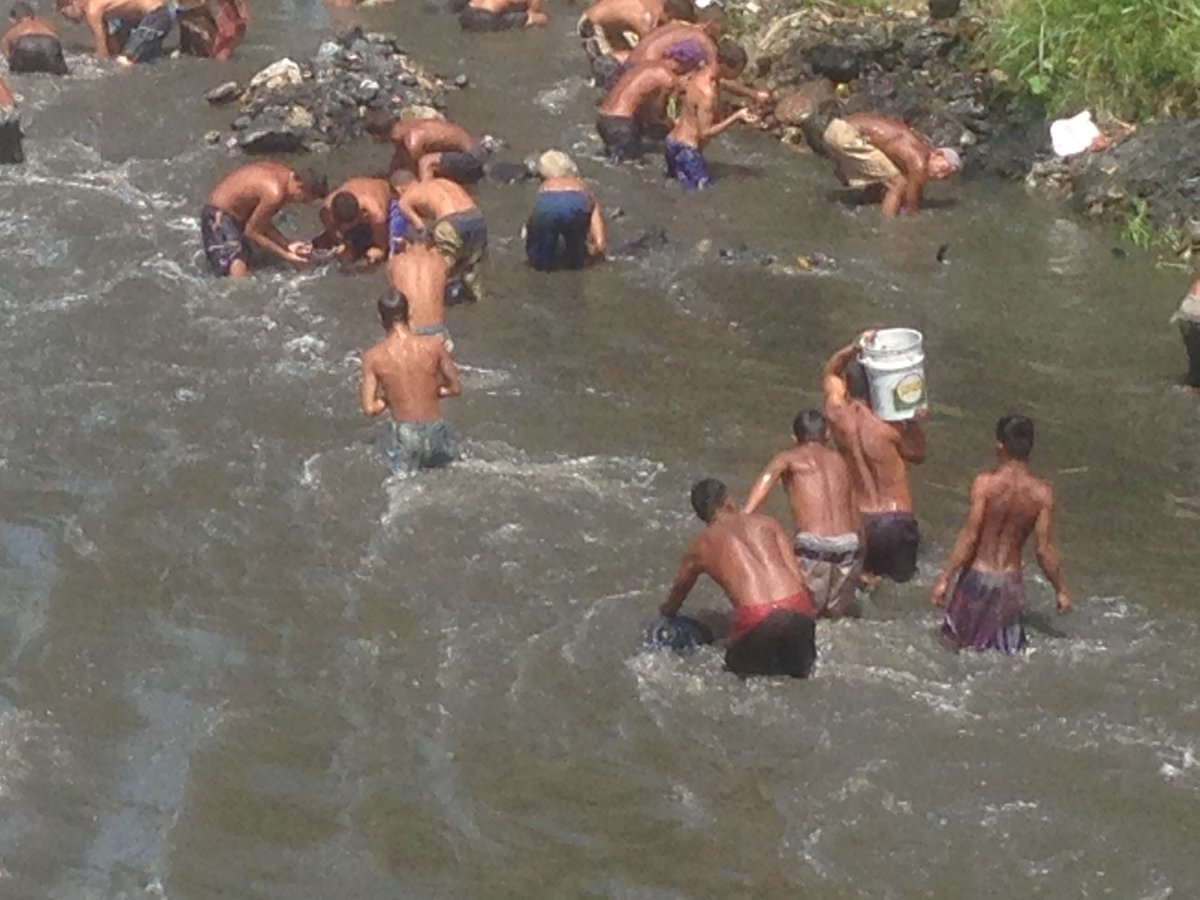
\includegraphics[width=300px]{20.jpg}%
\newline%
%
JESÚS A. HERRERA S.%
\newline%
%
Caracas.{-} Al menos 15 personas fueron retenidas por funcionarios de la Policía Nacional Bolivariana (PNB) en el módulo vial de Macaracuay este lunes por encontrarse dentro de las aguas contaminadas del río Guaire buscando objetos de valor, a la altura de El Llanito.%
\newline%
%
Los “garimpeiros” del Guaire dijeron que se encontraban buscando oro y otras piedras preciosas que eventualmente están sumergidas en el río, según la información del periodista Joan Camargo.%
\newline%
%
Algunos de estos vendrían de Charallave, estado Miranda, y procedieron a minar en el río Guaire porque en días anteriores otras personas lo hicieron y consiguieron objetos de valor.%
\newline%
%
Mientras dure la detención, las autoridades esperan hacerles un chequeo general y averiguar sus antecedentes y situación social.%
\newline%
%
\end{document}